\documentclass[12pt, a4paper]{article}
\usepackage[utf8]{inputenc}
\usepackage{graphicx}
\usepackage{geometry}
\usepackage{times}
\usepackage{url}
\usepackage{listings}
\usepackage{color}
\usepackage{caption}
\usepackage{subcaption}

\geometry{top=1in, bottom=1in, left=1in, right=1in}

\title{COL 334/672: Assignment 3 - Milestone 1 Report}
\author{Parth Thakur, 2021CS50615 \\ Amish Kansal, 2021CS50622}
\date{\today}

\begin{document}

\maketitle

\section{Introduction}
In this milestone, the goal was to send and receive UDP packets in accordance with the specified protocol. The server provided information about the total size of the data to be received. The client's task was to reliably receive the data, overcoming the challenges posed by a lossy network and the server's leaky bucket filtering mechanism.

\section{Implementation Details}
The code was written in Python, leveraging the socket and hashlib libraries. The client sends requests to the server and waits for a response. If no response is received within a specified timeout, the client resends the request.

\subsection{Reliable Data Reception}
To ensure the reliable reception of data, the client:
\begin{itemize}
    \item Sends a "SendSize" request to the server to get the total size of the data.
    \item Sequentially requests data packets starting from an offset. If the expected packet is not received or if the received packet's offset and size do not match the expected values, the client resends the request.
    \item Introduces sleep intervals between requests to avoid overwhelming the server.
\end{itemize}

\subsection{Hash Verification}
After receiving all the data packets, the client computes the MD5 hash of the received data and sends it to the server for verification.

\subsection{Graphical Analysis}
The client logs the time and offset for each data request sent and received. This data is used to generate graphs showing the sequence-number trace and a zoomed-in view of the trace.

\section{Results and Observations}
The attached figures show the sequence-number trace and its zoomed-in view. The blue dots represent the time and offset of the requests sent by the client, while the orange dots represent the corresponding replies received from the server.

\begin{figure}[h]
\centering
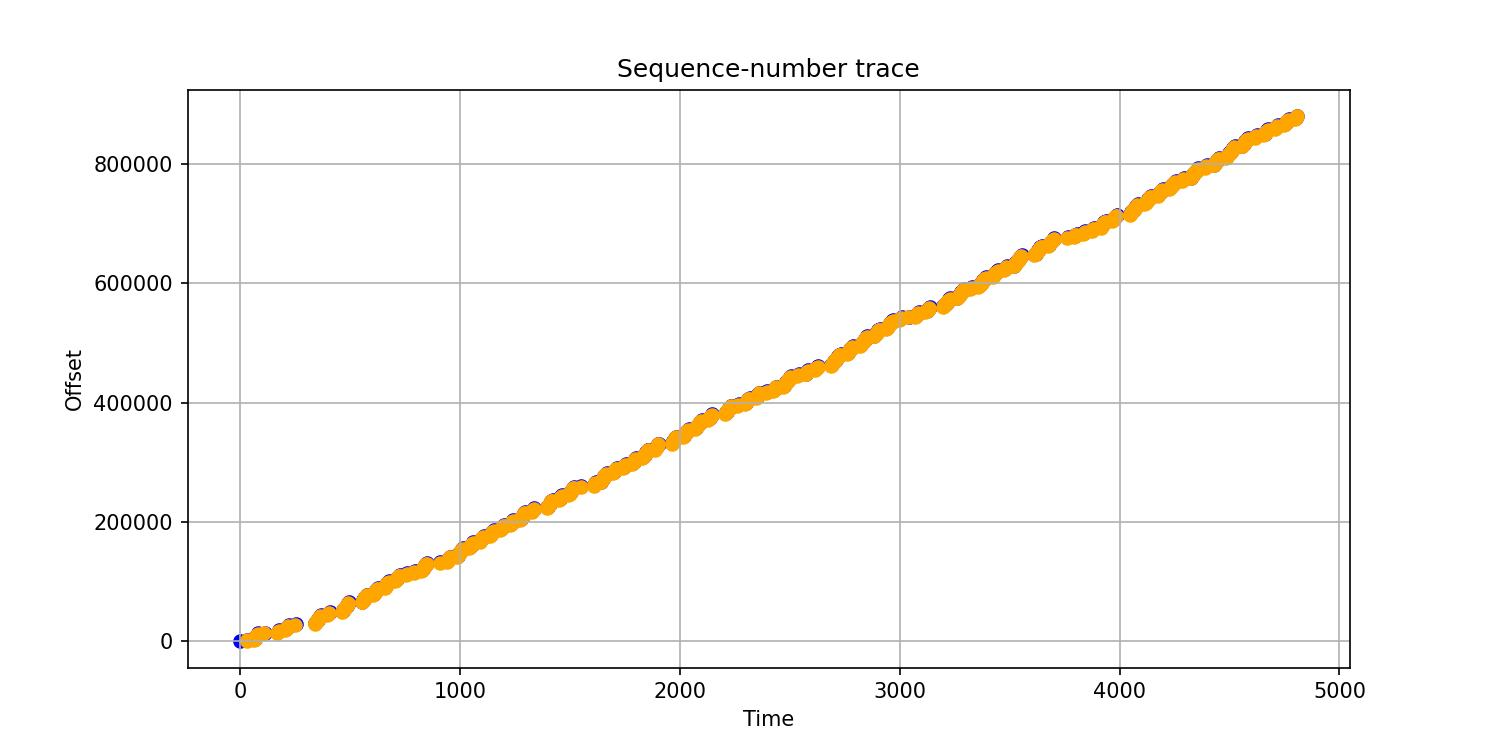
\includegraphics[width=0.9\linewidth]{Sequence-number trace.jpeg}
\caption{Sequence-number trace}
\label{fig:sequence_trace}
\end{figure}

\begin{figure}[h]
\centering
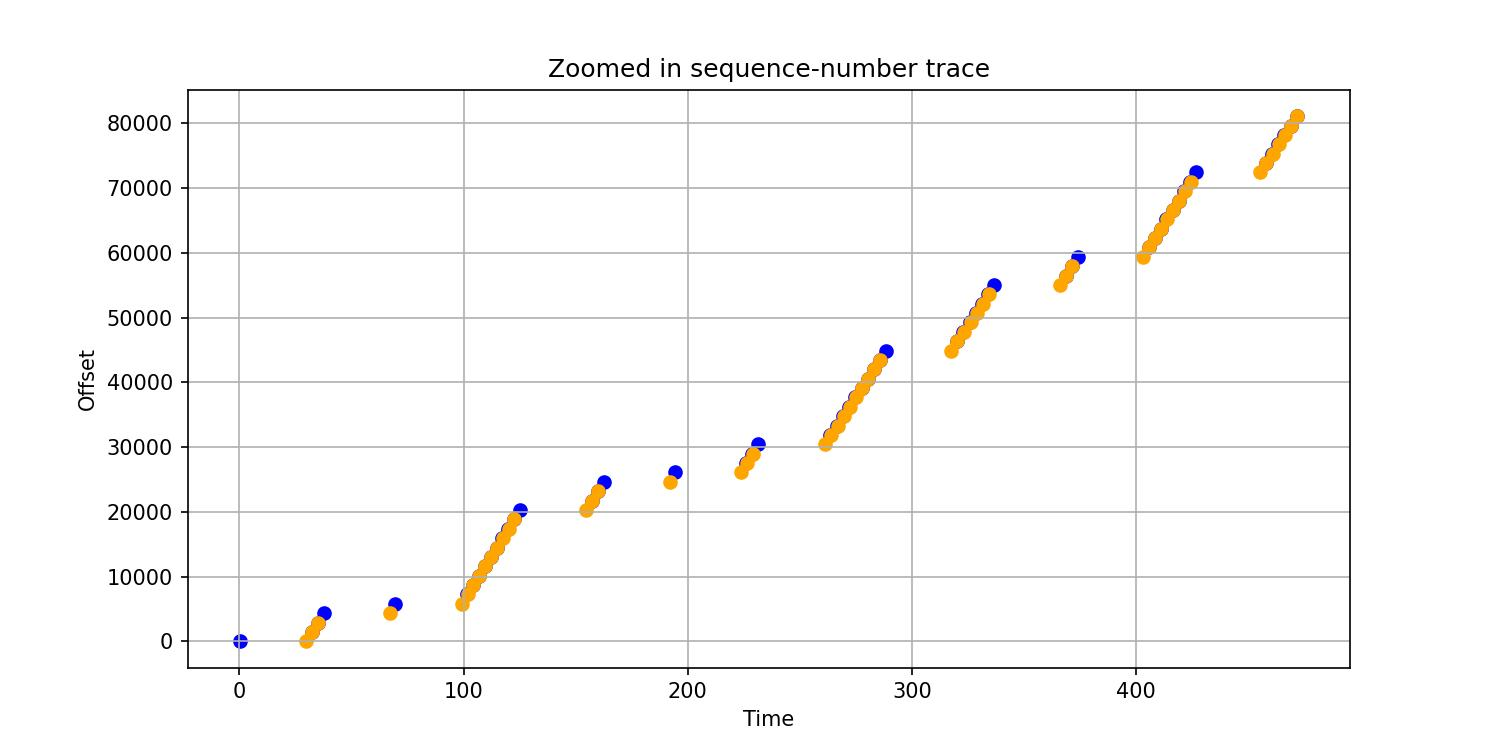
\includegraphics[width=0.9\linewidth]{Zoomed in sequence-number trace.jpeg}
\caption{Zoomed in sequence-number trace}
\label{fig:zoomed_trace}
\end{figure}

\section{Conclusion}
The client was able to reliably receive data from the server by retransmitting requests when necessary and adjusting the request rate to avoid overwhelming the server. The generated graphs provided insights into the client-server interaction dynamics and the reliability mechanisms in place.

\section{Future Work}
For the upcoming milestones, the focus will be on optimizing the request rate to maximize throughput without getting "squished" by the server's leaky bucket filter and on handling variable server rates.

\end{document}
